\chapter{Algoritmi na stablima}

\index{stablo}

\key{Stablo} je povezan graf bez ciklusa
koji se sastoji od $n$ čvorova i $n-1$ bridova.
Uklanjanje bilo kojeg brida iz stabla dijeli ga
na dvije komponente,
a dodavanje bilo kojeg brida u stablo stvara ciklus.
Štoviše, između bilo koja dva
čvora stabla uvijek postoji jedinstven put.

Na primjer, sljedeće stablo sastoji se od 8 čvorova i 7 bridova:
\begin{center}
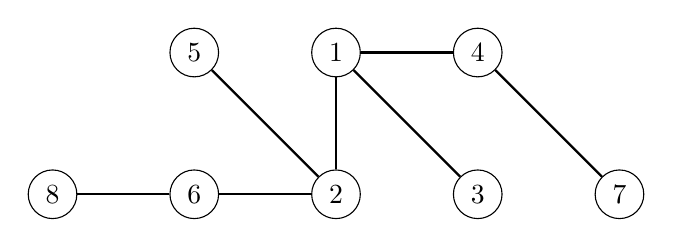
\begin{tikzpicture}[scale=0.9]
\node[draw, circle] (1) at (0,3) {$1$};
\node[draw, circle] (2) at (2,3) {$4$};
\node[draw, circle] (3) at (0,1) {$2$};
\node[draw, circle] (4) at (2,1) {$3$};
\node[draw, circle] (5) at (4,1) {$7$};
\node[draw, circle] (6) at (-2,3) {$5$};
\node[draw, circle] (7) at (-2,1) {$6$};
\node[draw, circle] (8) at (-4,1) {$8$};
\path[draw,thick,-] (1) -- (2);
\path[draw,thick,-] (1) -- (3);
\path[draw,thick,-] (1) -- (4);
\path[draw,thick,-] (2) -- (5);
\path[draw,thick,-] (3) -- (6);
\path[draw,thick,-] (3) -- (7);
\path[draw,thick,-] (7) -- (8);
\end{tikzpicture}
\end{center}

\index{list}

\key{Listovi} stabla su čvorovi
stupnja 1, tj. oni koji imaju samo jednog susjeda.
Na primjer, listovi gornjeg stabla
su čvorovi 3, 5, 7 i 8.

\index{korijen}
\index{ukorijenjeno stablo}

U \key{ukorijenjenom} stablu jedan od čvorova
proglašen je \key{korijenom} stabla,
a svi ostali čvorovi
smješteni su ispod korijena.
Na primjer, u sljedećem stablu
čvor 1 je korijenski čvor.

\begin{center}
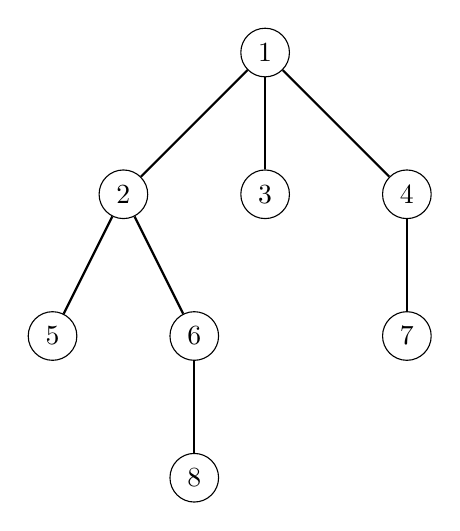
\begin{tikzpicture}[scale=0.9]
\node[draw, circle] (1) at (0,3) {$1$};
\node[draw, circle] (4) at (2,1) {$4$};
\node[draw, circle] (2) at (-2,1) {$2$};
\node[draw, circle] (3) at (0,1) {$3$};
\node[draw, circle] (7) at (2,-1) {$7$};
\node[draw, circle] (5) at (-3,-1) {$5$};
\node[draw, circle] (6) at (-1,-1) {$6$};
\node[draw, circle] (8) at (-1,-3) {$8$};
\path[draw,thick,-] (1) -- (2);
\path[draw,thick,-] (1) -- (3);
\path[draw,thick,-] (1) -- (4);
\path[draw,thick,-] (2) -- (5);
\path[draw,thick,-] (2) -- (6);
\path[draw,thick,-] (4) -- (7);
\path[draw,thick,-] (6) -- (8);
\end{tikzpicture}
\end{center}
\index{dijete}
\index{roditelj}

U ukorijenjenom stablu \key{djeca} čvora
su njegovi donji susjedi, a \key{roditelj} čvora
je njegov gornji susjed.
Svaki čvor ima točno jednog roditelja,
osim korijena koji nema roditelja.
Na primjer, u gornjem stablu
djeca čvora 2 su čvorovi 5 i 6,
a njegov roditelj je čvor 1.

\index{podstablo}

Struktura ukorijenjenog stabla je \emph{rekurzivna}:
svaki čvor stabla djeluje kao korijen \key{podstabla}
koje sadrži sam čvor i sve čvorove
koji se nalaze u podstablima njegove djece.
Na primjer, u gornjem stablu podstablo čvora 2
sastoji se od čvorova 2, 5, 6 i 8:
\begin{center}
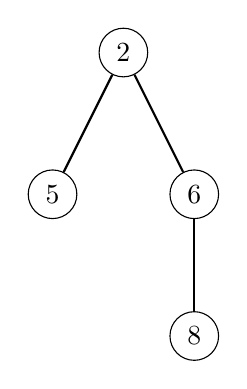
\begin{tikzpicture}[scale=0.9]
\node[draw, circle] (2) at (-2,1) {$2$};
\node[draw, circle] (5) at (-3,-1) {$5$};
\node[draw, circle] (6) at (-1,-1) {$6$};
\node[draw, circle] (8) at (-1,-3) {$8$};
\path[draw,thick,-] (2) -- (5);
\path[draw,thick,-] (2) -- (6);
\path[draw,thick,-] (6) -- (8);
\end{tikzpicture}
\end{center}

\section{Obilazak stabla}

Za obilazak čvorova stabla mogu se koristiti
opći algoritmi za obilazak grafova.
Međutim, obilazak stabla lakše je implementirati nego
obilazak općeg grafa jer
u stablu nema ciklusa i nije
moguće doći do čvora iz više smjerova.

Uobičajen način obilaska stabla je pokretanje
pretraživanja u dubinu iz proizvoljnog čvora.
Može se koristiti sljedeća rekurzivna funkcija:

\begin{lstlisting}
void dfs(int s, int e) {
    // obradi čvor s
    cout << s << " ";
    for (auto u : adj[s]) {
        if (u != e) dfs(u, s);
    }
}
\end{lstlisting}

Funkcija dobiva dva parametra: trenutni čvor $s$
i prethodni čvor $e$.
Svrha parametra $e$ je osigurati
da se pretraživanje pomiče samo na čvorove
koji još nisu posjećeni.

Sljedeći poziv funkcije pokreće pretraživanje
u čvoru $x$:

\begin{lstlisting}
dfs(x, 0);
\end{lstlisting}

U prvom pozivu je $e=0$ jer nema
prethodnog čvora, pa je dopušteno
nastaviti u bilo kojem smjeru u stablu.

\subsubsection{Dinamičko programiranje}

Dinamičko programiranje može se koristiti za izračun
nekih informacija tijekom obilaska stabla.
Pomoću dinamičkog programiranja možemo, na primjer,
u $O(n)$ vremenu za svaki čvor ukorijenjenog stabla izračunati
broj čvorova u njegovu podstablu
ili duljinu najduljeg puta od čvora
do lista.

Kao primjer, izračunajmo za svaki čvor $s$
vrijednost $\texttt{count}[s]$: broj čvorova u njegovu podstablu.
Podstablo sadrži sam čvor i
sve čvorove u podstablima njegove djece,
pa broj čvorova možemo izračunati
rekurzivno pomoću sljedećeg koda:

\begin{lstlisting}
void dfs(int s, int e) {
    count[s] = 1;
    for (auto u : adj[s]) {
        if (u == e) continue;
        dfs(u, s);
        count[s] += count[u];
    }
}
\end{lstlisting}

\section{Promjer}

\index{promjer}

\key{Promjer} stabla
je najveća duljina puta između dva čvora.
Na primjer, razmotrimo sljedeće stablo:
\begin{center}
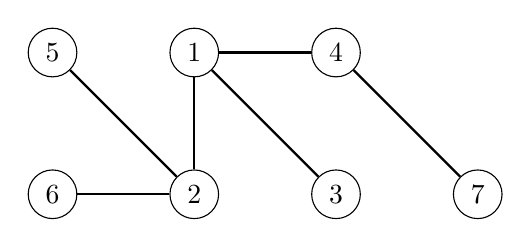
\begin{tikzpicture}[scale=0.9]
\node[draw, circle] (1) at (0,3) {$1$};
\node[draw, circle] (2) at (2,3) {$4$};
\node[draw, circle] (3) at (0,1) {$2$};
\node[draw, circle] (4) at (2,1) {$3$};
\node[draw, circle] (5) at (4,1) {$7$};
\node[draw, circle] (6) at (-2,3) {$5$};
\node[draw, circle] (7) at (-2,1) {$6$};
\path[draw,thick,-] (1) -- (2);
\path[draw,thick,-] (1) -- (3);
\path[draw,thick,-] (1) -- (4);
\path[draw,thick,-] (2) -- (5);
\path[draw,thick,-] (3) -- (6);
\path[draw,thick,-] (3) -- (7);
\end{tikzpicture}
\end{center}
Promjer ovog stabla je 4,
što odgovara sljedećem putu:
\begin{center}
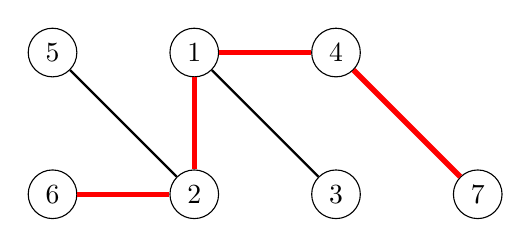
\begin{tikzpicture}[scale=0.9]
\node[draw, circle] (1) at (0,3) {$1$};
\node[draw, circle] (2) at (2,3) {$4$};
\node[draw, circle] (3) at (0,1) {$2$};
\node[draw, circle] (4) at (2,1) {$3$};
\node[draw, circle] (5) at (4,1) {$7$};
\node[draw, circle] (6) at (-2,3) {$5$};
\node[draw, circle] (7) at (-2,1) {$6$};
\path[draw,thick,-] (1) -- (2);
\path[draw,thick,-] (1) -- (3);
\path[draw,thick,-] (1) -- (4);
\path[draw,thick,-] (2) -- (5);
\path[draw,thick,-] (3) -- (6);
\path[draw,thick,-] (3) -- (7);

\path[draw,thick,-,color=red,line width=2pt] (7) -- (3);
\path[draw,thick,-,color=red,line width=2pt] (3) -- (1);
\path[draw,thick,-,color=red,line width=2pt] (1) -- (2);
\path[draw,thick,-,color=red,line width=2pt] (2) -- (5);
\end{tikzpicture}
\end{center}
Primijetimo da može postojati više puteva maksimalne duljine.
U gornjem putu mogli bismo zamijeniti čvor 6 čvorom 5
i dobiti drugi put duljine 4.

Zatim ćemo razmotriti dva algoritma s vremenskom složenošću $O(n)$
za izračun promjera stabla.
Prvi algoritam temelji se na dinamičkom programiranju,
a drugi algoritam koristi dva pretraživanja u dubinu.

\subsubsection{Algoritam 1}

Općenit način pristupa mnogim zadacima na stablima
je da stablo najprije proizvoljno ukorijenimo.
Nakon toga možemo pokušati riješiti zadatak
zasebno za svako podstablo.
Naš prvi algoritam za izračun promjera
temelji se na toj ideji.

Važno je uočiti da svaki put
u ukorijenjenom stablu ima \emph{najvišu točku}:
najviši čvor koji pripada tom putu.
Stoga za svaki čvor možemo izračunati duljinu
najduljeg puta čija je najviša točka taj čvor.
Jedan od tih puteva odgovara promjeru stabla.

Na primjer, u sljedećem stablu
čvor 1 je najviša točka na putu
koji odgovara promjeru:
\begin{center}
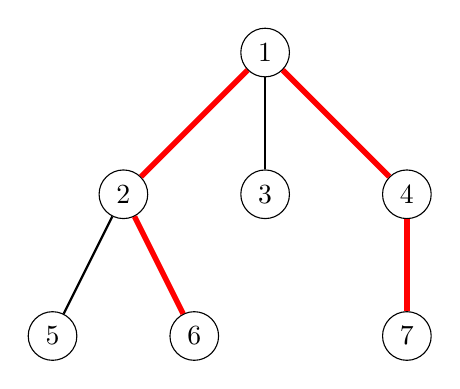
\begin{tikzpicture}[scale=0.9]
\node[draw, circle] (1) at (0,3) {$1$};
\node[draw, circle] (2) at (2,1) {$4$};
\node[draw, circle] (3) at (-2,1) {$2$};
\node[draw, circle] (4) at (0,1) {$3$};
\node[draw, circle] (5) at (2,-1) {$7$};
\node[draw, circle] (6) at (-3,-1) {$5$};
\node[draw, circle] (7) at (-1,-1) {$6$};
\path[draw,thick,-] (1) -- (2);
\path[draw,thick,-] (1) -- (3);
\path[draw,thick,-] (1) -- (4);
\path[draw,thick,-] (2) -- (5);
\path[draw,thick,-] (3) -- (6);
\path[draw,thick,-] (3) -- (7);

\path[draw,thick,-,color=red,line width=2pt] (7) -- (3);
\path[draw,thick,-,color=red,line width=2pt] (3) -- (1);
\path[draw,thick,-,color=red,line width=2pt] (1) -- (2);
\path[draw,thick,-,color=red,line width=2pt] (2) -- (5);
\end{tikzpicture}
\end{center}

Za svaki čvor $x$ računamo dvije vrijednosti:
\begin{itemize}
\item $\texttt{toLeaf}(x)$: najveća duljina puta od $x$ do bilo kojeg lista
\item $\texttt{maxLength}(x)$: najveća duljina puta
čija je najviša točka $x$
\end{itemize}
Na primjer, u gornjem stablu je
$\texttt{toLeaf}(1)=2$ jer postoji put
$1 \rightarrow 2 \rightarrow 6$,
i $\texttt{maxLength}(1)=4$
jer postoji put
$6 \rightarrow 2 \rightarrow 1 \rightarrow 4 \rightarrow 7$.
U ovom slučaju $\texttt{maxLength}(1)$ jednak je promjeru.

Dinamičko programiranje može se koristiti za izračun gornjih
vrijednosti za sve čvorove u $O(n)$ vremenu.
Najprije, da bismo izračunali $\texttt{toLeaf}(x)$,
prolazimo kroz djecu čvora $x$,
biramo dijete $c$ s najvećom vrijednošću $\texttt{toLeaf}(c)$
i toj vrijednosti dodajemo jedan.
Zatim, da bismo izračunali $\texttt{maxLength}(x)$,
biramo dva različita djeteta $a$ i $b$
takva da je suma $\texttt{toLeaf}(a)+\texttt{toLeaf}(b)$
najveća te toj sumi dodajemo dva.

\subsubsection{Algoritam 2}

Drugi efikasan način izračuna promjera
stabla temelji se na dva pretraživanja u dubinu.
Najprije odaberemo proizvoljan čvor $a$ u stablu
i pronađemo najudaljeniji čvor $b$ od $a$.
Zatim pronađemo najudaljeniji čvor $c$ od $b$.
Promjer stabla je udaljenost između $b$ i $c$.

U sljedećem grafu $a$, $b$ i $c$ mogli bi biti:
\begin{center}
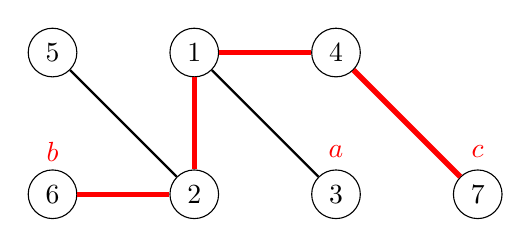
\begin{tikzpicture}[scale=0.9]
\node[draw, circle] (1) at (0,3) {$1$};
\node[draw, circle] (2) at (2,3) {$4$};
\node[draw, circle] (3) at (0,1) {$2$};
\node[draw, circle] (4) at (2,1) {$3$};
\node[draw, circle] (5) at (4,1) {$7$};
\node[draw, circle] (6) at (-2,3) {$5$};
\node[draw, circle] (7) at (-2,1) {$6$};
\path[draw,thick,-] (1) -- (2);
\path[draw,thick,-] (1) -- (3);
\path[draw,thick,-] (1) -- (4);
\path[draw,thick,-] (2) -- (5);
\path[draw,thick,-] (3) -- (6);
\path[draw,thick,-] (3) -- (7);
\node[color=red] at (2,1.6) {$a$};
\node[color=red] at (-2,1.6) {$b$};
\node[color=red] at (4,1.6) {$c$};

\path[draw,thick,-,color=red,line width=2pt] (7) -- (3);
\path[draw,thick,-,color=red,line width=2pt] (3) -- (1);
\path[draw,thick,-,color=red,line width=2pt] (1) -- (2);
\path[draw,thick,-,color=red,line width=2pt] (2) -- (5);
\end{tikzpicture}
\end{center}

Ovo je elegantna metoda, ali zašto ona radi?

Pomaže nacrtati stablo drukčije tako da
put koji odgovara promjeru
bude vodoravan, a svi ostali
čvorovi vise s njega:
\begin{center}
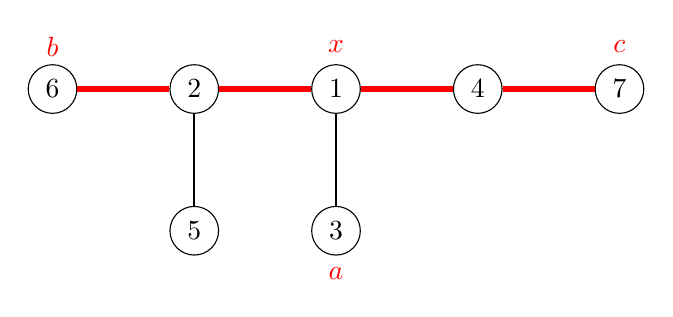
\begin{tikzpicture}[scale=0.9]
\node[draw, circle] (1) at (2,1) {$1$};
\node[draw, circle] (2) at (4,1) {$4$};
\node[draw, circle] (3) at (0,1) {$2$};
\node[draw, circle] (4) at (2,-1) {$3$};
\node[draw, circle] (5) at (6,1) {$7$};
\node[draw, circle] (6) at (0,-1) {$5$};
\node[draw, circle] (7) at (-2,1) {$6$};
\path[draw,thick,-] (1) -- (2);
\path[draw,thick,-] (1) -- (3);
\path[draw,thick,-] (1) -- (4);
\path[draw,thick,-] (2) -- (5);
\path[draw,thick,-] (3) -- (6);
\path[draw,thick,-] (3) -- (7);
\node[color=red] at (2,-1.6) {$a$};
\node[color=red] at (-2,1.6) {$b$};
\node[color=red] at (6,1.6) {$c$};
\node[color=red] at (2,1.6) {$x$};

\path[draw,thick,-,color=red,line width=2pt] (7) -- (3);
\path[draw,thick,-,color=red,line width=2pt] (3) -- (1);
\path[draw,thick,-,color=red,line width=2pt] (1) -- (2);
\path[draw,thick,-,color=red,line width=2pt] (2) -- (5);
\end{tikzpicture}
\end{center}

Čvor $x$ označava mjesto na kojem se put
od čvora $a$ spaja s putem koji odgovara
promjeru.
Najudaljeniji čvor od $a$
je čvor $b$, čvor $c$ ili neki drugi čvor
koji je barem jednako udaljen od čvora $x$.
Stoga je taj čvor uvijek valjan izbor za
krajnju točku puta koji odgovara promjeru.

\section{Svi najdulji putevi}

Naš sljedeći zadatak je izračunati za svaki čvor
u stablu najveću duljinu puta
koji počinje u tom čvoru.
To se može promatrati kao poopćenje
zadatka o promjeru stabla jer je najveća od tih
duljina jednaka promjeru stabla.
I ovaj se zadatak može riješiti u $O(n)$ vremenu.

Kao primjer, razmotrimo sljedeće stablo:
\begin{center}
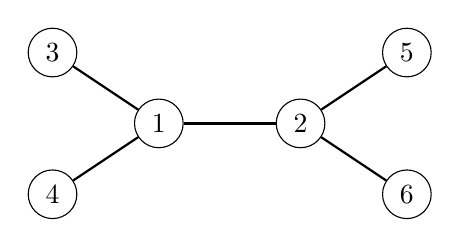
\begin{tikzpicture}[scale=0.9]
\node[draw, circle] (1) at (0,0) {$1$};
\node[draw, circle] (2) at (-1.5,-1) {$4$};
\node[draw, circle] (3) at (2,0) {$2$};
\node[draw, circle] (4) at (-1.5,1) {$3$};
\node[draw, circle] (6) at (3.5,-1) {$6$};
\node[draw, circle] (7) at (3.5,1) {$5$};
\path[draw,thick,-] (1) -- (2);
\path[draw,thick,-] (1) -- (3);
\path[draw,thick,-] (1) -- (4);
\path[draw,thick,-] (3) -- (6);
\path[draw,thick,-] (3) -- (7);
\end{tikzpicture}
\end{center}

Neka $\texttt{maxLength}(x)$ označava najveću duljinu
puta koji počinje u čvoru $x$.
Na primjer, u gornjem stablu je
$\texttt{maxLength}(4)=3$ jer postoji
put $4 \rightarrow 1 \rightarrow 2 \rightarrow 6$.
Evo potpune tablice vrijednosti:
\begin{center}
\begin{tabular}{l|lllllll}
čvor $x$ & 1 & 2 & 3 & 4 & 5 & 6 \\
$\texttt{maxLength}(x)$ & 2 & 2 & 3 & 3 & 3 & 3 \\
\end{tabular}
\end{center}

I u ovom zadatku dobra polazna točka
za rješavanje je proizvoljno ukorijeniti stablo:
\begin{center}
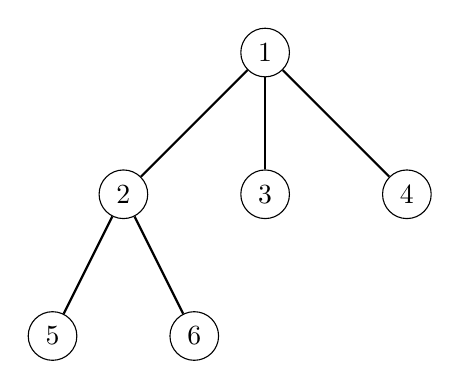
\begin{tikzpicture}[scale=0.9]
\node[draw, circle] (1) at (0,3) {$1$};
\node[draw, circle] (2) at (2,1) {$4$};
\node[draw, circle] (3) at (-2,1) {$2$};
\node[draw, circle] (4) at (0,1) {$3$};
\node[draw, circle] (6) at (-3,-1) {$5$};
\node[draw, circle] (7) at (-1,-1) {$6$};
\path[draw,thick,-] (1) -- (2);
\path[draw,thick,-] (1) -- (3);
\path[draw,thick,-] (1) -- (4);
\path[draw,thick,-] (3) -- (6);
\path[draw,thick,-] (3) -- (7);
\end{tikzpicture}
\end{center}

Prvi dio zadatka je izračunati za svaki čvor $x$
najveću duljinu puta koji prolazi kroz neko dijete čvora $x$.
Na primjer, najdulji put iz čvora 1
prolazi kroz njegovo dijete 2:
\begin{center}
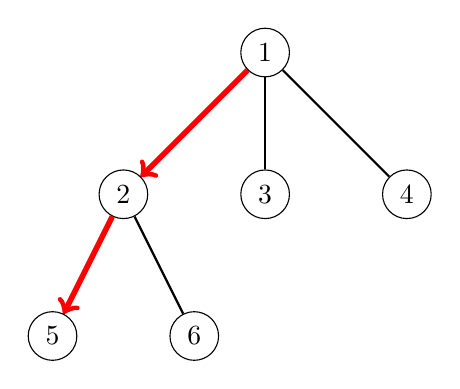
\begin{tikzpicture}[scale=0.9]
\node[draw, circle] (1) at (0,3) {$1$};
\node[draw, circle] (2) at (2,1) {$4$};
\node[draw, circle] (3) at (-2,1) {$2$};
\node[draw, circle] (4) at (0,1) {$3$};
\node[draw, circle] (6) at (-3,-1) {$5$};
\node[draw, circle] (7) at (-1,-1) {$6$};
\path[draw,thick,-] (1) -- (2);
\path[draw,thick,-] (1) -- (3);
\path[draw,thick,-] (1) -- (4);
\path[draw,thick,-] (3) -- (6);
\path[draw,thick,-] (3) -- (7);

\path[draw,thick,->,color=red,line width=2pt] (1) -- (3);
\path[draw,thick,->,color=red,line width=2pt] (3) -- (6);
\end{tikzpicture}
\end{center}
Taj je dio lako riješiti u $O(n)$ vremenu jer možemo koristiti
dinamičko programiranje kao što smo radili i prije.

Zatim, drugi dio zadatka je izračunati
za svaki čvor $x$ najveću duljinu puta
koji prolazi kroz njegova roditelja $p$.
Na primjer, najdulji put
iz čvora 3 prolazi kroz njegova roditelja 1:
\begin{center}
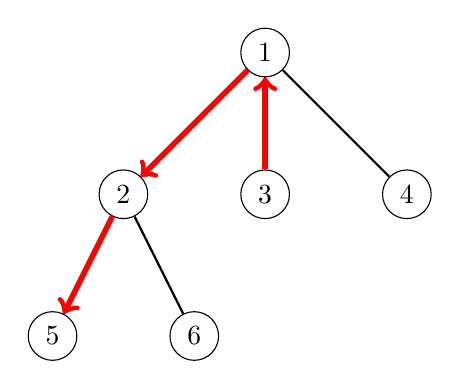
\begin{tikzpicture}[scale=0.9]
\node[draw, circle] (1) at (0,3) {$1$};
\node[draw, circle] (2) at (2,1) {$4$};
\node[draw, circle] (3) at (-2,1) {$2$};
\node[draw, circle] (4) at (0,1) {$3$};
\node[draw, circle] (6) at (-3,-1) {$5$};
\node[draw, circle] (7) at (-1,-1) {$6$};
\path[draw,thick,-] (1) -- (2);
\path[draw,thick,-] (1) -- (3);
\path[draw,thick,-] (1) -- (4);
\path[draw,thick,-] (3) -- (6);
\path[draw,thick,-] (3) -- (7);

\path[draw,thick,->,color=red,line width=2pt] (4) -- (1);
\path[draw,thick,->,color=red,line width=2pt] (1) -- (3);
\path[draw,thick,->,color=red,line width=2pt] (3) -- (6);
\end{tikzpicture}
\end{center}

Na prvi pogled čini se da bismo trebali odabrati
najdulji put iz $p$.
Međutim, to \emph{ne} radi uvijek
jer najdulji put iz $p$
može prolaziti kroz $x$.
Evo primjera takve situacije:
\begin{center}
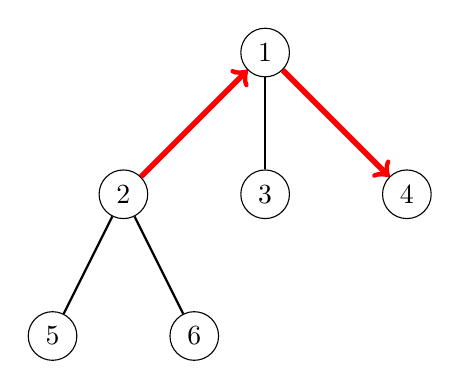
\begin{tikzpicture}[scale=0.9]
\node[draw, circle] (1) at (0,3) {$1$};
\node[draw, circle] (2) at (2,1) {$4$};
\node[draw, circle] (3) at (-2,1) {$2$};
\node[draw, circle] (4) at (0,1) {$3$};
\node[draw, circle] (6) at (-3,-1) {$5$};
\node[draw, circle] (7) at (-1,-1) {$6$};
\path[draw,thick,-] (1) -- (2);
\path[draw,thick,-] (1) -- (3);
\path[draw,thick,-] (1) -- (4);
\path[draw,thick,-] (3) -- (6);
\path[draw,thick,-] (3) -- (7);

\path[draw,thick,->,color=red,line width=2pt] (3) -- (1);
\path[draw,thick,->,color=red,line width=2pt] (1) -- (2);
\end{tikzpicture}
\end{center}

Ipak, drugi dio možemo riješiti u
$O(n)$ vremenu tako da pohranimo \emph{dvije} najveće duljine
za svaki čvor $x$:
\begin{itemize}
\item $\texttt{maxLength}_1(x)$:
najveća duljina puta iz $x$
\item $\texttt{maxLength}_2(x)$
najveća duljina puta iz $x$
u smjeru različitom od smjera prvog puta
\end{itemize}
Na primjer, u gornjem grafu je
$\texttt{maxLength}_1(1)=2$
koristeći put $1 \rightarrow 2 \rightarrow 5$,
i $\texttt{maxLength}_2(1)=1$
koristeći put $1 \rightarrow 3$.

Konačno, ako put koji odgovara
vrijednosti $\texttt{maxLength}_1(p)$ prolazi kroz $x$,
zaključujemo da je najveća duljina
$\texttt{maxLength}_2(p)+1$,
a inače je najveća duljina
$\texttt{maxLength}_1(p)+1$.


\section{Binarna stabla}

\index{binarno stablo}

\begin{samepage}
\key{Binarno stablo} je ukorijenjeno stablo
u kojem svaki čvor ima lijevo i desno podstablo.
Moguće je da je neko podstablo čvora prazno.
Stoga svaki čvor u binarnom stablu ima
nula, jedno ili dvoje djece.

Na primjer, sljedeće stablo je binarno stablo:
\begin{center}
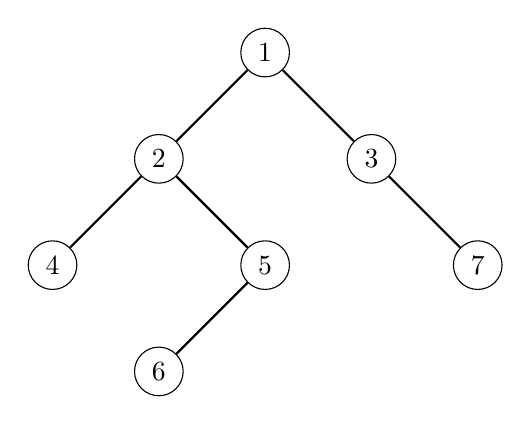
\begin{tikzpicture}[scale=0.9]
\node[draw, circle] (1) at (0,0) {$1$};
\node[draw, circle] (2) at (-1.5,-1.5) {$2$};
\node[draw, circle] (3) at (1.5,-1.5) {$3$};
\node[draw, circle] (4) at (-3,-3) {$4$};
\node[draw, circle] (5) at (0,-3) {$5$};
\node[draw, circle] (6) at (-1.5,-4.5) {$6$};
\node[draw, circle] (7) at (3,-3) {$7$};

\path[draw,thick,-] (1) -- (2);
\path[draw,thick,-] (1) -- (3);
\path[draw,thick,-] (2) -- (4);
\path[draw,thick,-] (2) -- (5);
\path[draw,thick,-] (5) -- (6);
\path[draw,thick,-] (3) -- (7);
\end{tikzpicture}
\end{center}
\end{samepage}

\index{preorder}
\index{inorder}
\index{postorder}

Čvorovi binarnog stabla imaju tri prirodna
poretka koji odgovaraju različitim načinima 
rekurzivnog obilaska stabla:

\begin{itemize}
\item \key{preorder}: najprije obradi korijen,
zatim obiđi lijevo podstablo, pa obiđi desno podstablo
\item \key{inorder}: najprije obiđi lijevo podstablo,
zatim obradi korijen, pa obiđi desno podstablo
\item \key{postorder}: najprije obiđi lijevo podstablo,
zatim obiđi desno podstablo, pa obradi korijen
\end{itemize}

Za gornje stablo čvorovi su u
preorder poretku
$[1,2,4,5,6,3,7]$,
u inorder poretku $[4,2,6,5,1,3,7]$,
a u postorder poretku $[4,6,5,2,7,3,1]$.

Ako znamo preorder i inorder poredak
stabla, možemo rekonstruirati točnu strukturu stabla.
Na primjer, gornje stablo je jedino moguće stablo
s preorder poretkom $[1,2,4,5,6,3,7]$ i
inorder poretkom $[4,2,6,5,1,3,7]$.
Na sličan način, postorder i inorder poredak
također određuju strukturu stabla.

Međutim, situacija je drukčija ako znamo samo
preorder i postorder poredak stabla.
U tom slučaju može postojati više od jednog stabla
koje odgovara tim poredcima.
Na primjer, u oba sljedeća stabla
\begin{center}
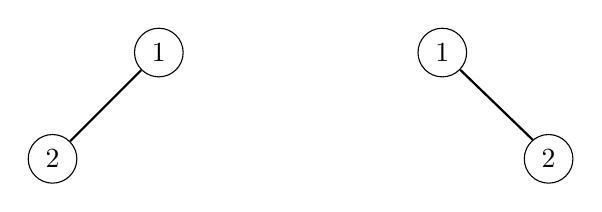
\begin{tikzpicture}[scale=0.9]
\node[draw, circle] (1) at (0,0) {$1$};
\node[draw, circle] (2) at (-1.5,-1.5) {$2$};
\path[draw,thick,-] (1) -- (2);

\node[draw, circle] (1b) at (0+4,0) {$1$};
\node[draw, circle] (2b) at (1.5+4,-1.5) {$2$};
\path[draw,thick,-] (1b) -- (2b);
\end{tikzpicture}
\end{center}
preorder poredak je $[1,2]$, a postorder poredak je $[2,1]$,
ali strukture stabala su različite.

